\section{Sattelite images}
The \srgui supports fetching sattelite images from the Norwegian Mapping Authority (Kartverket) use it as an overlay in the Map page as shown in Figure \ref{fig:gui_map} \cite{kartverketNorgeskart}.
The main intended use is to visualize from where each image are taken and ease the development future pose estimation systems.

\begin{figure}[H]
    \centering
    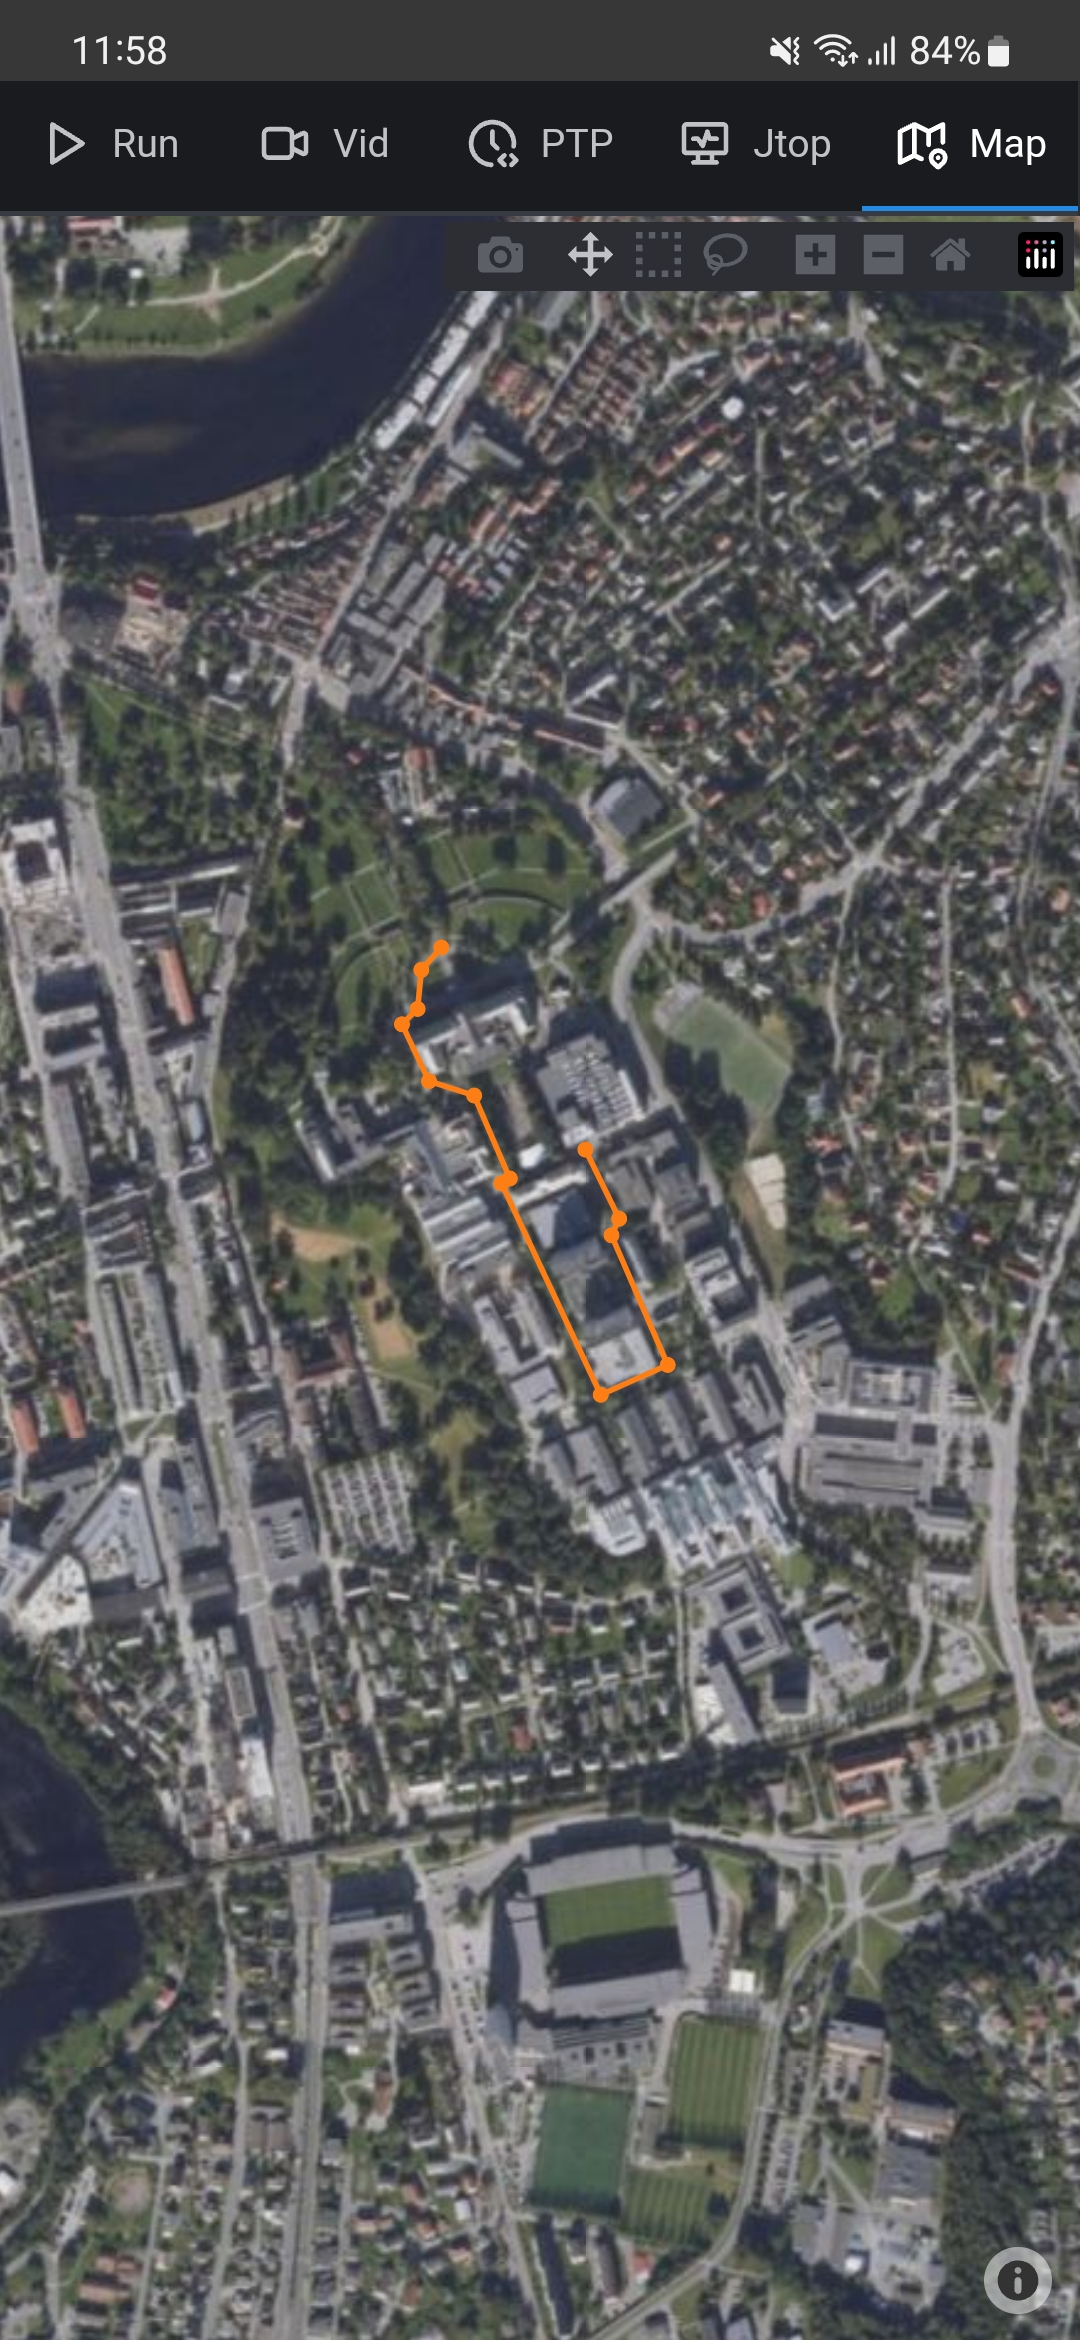
\includegraphics[width=.48\textwidth]{figures/gui/map_sattelite.jpg}
    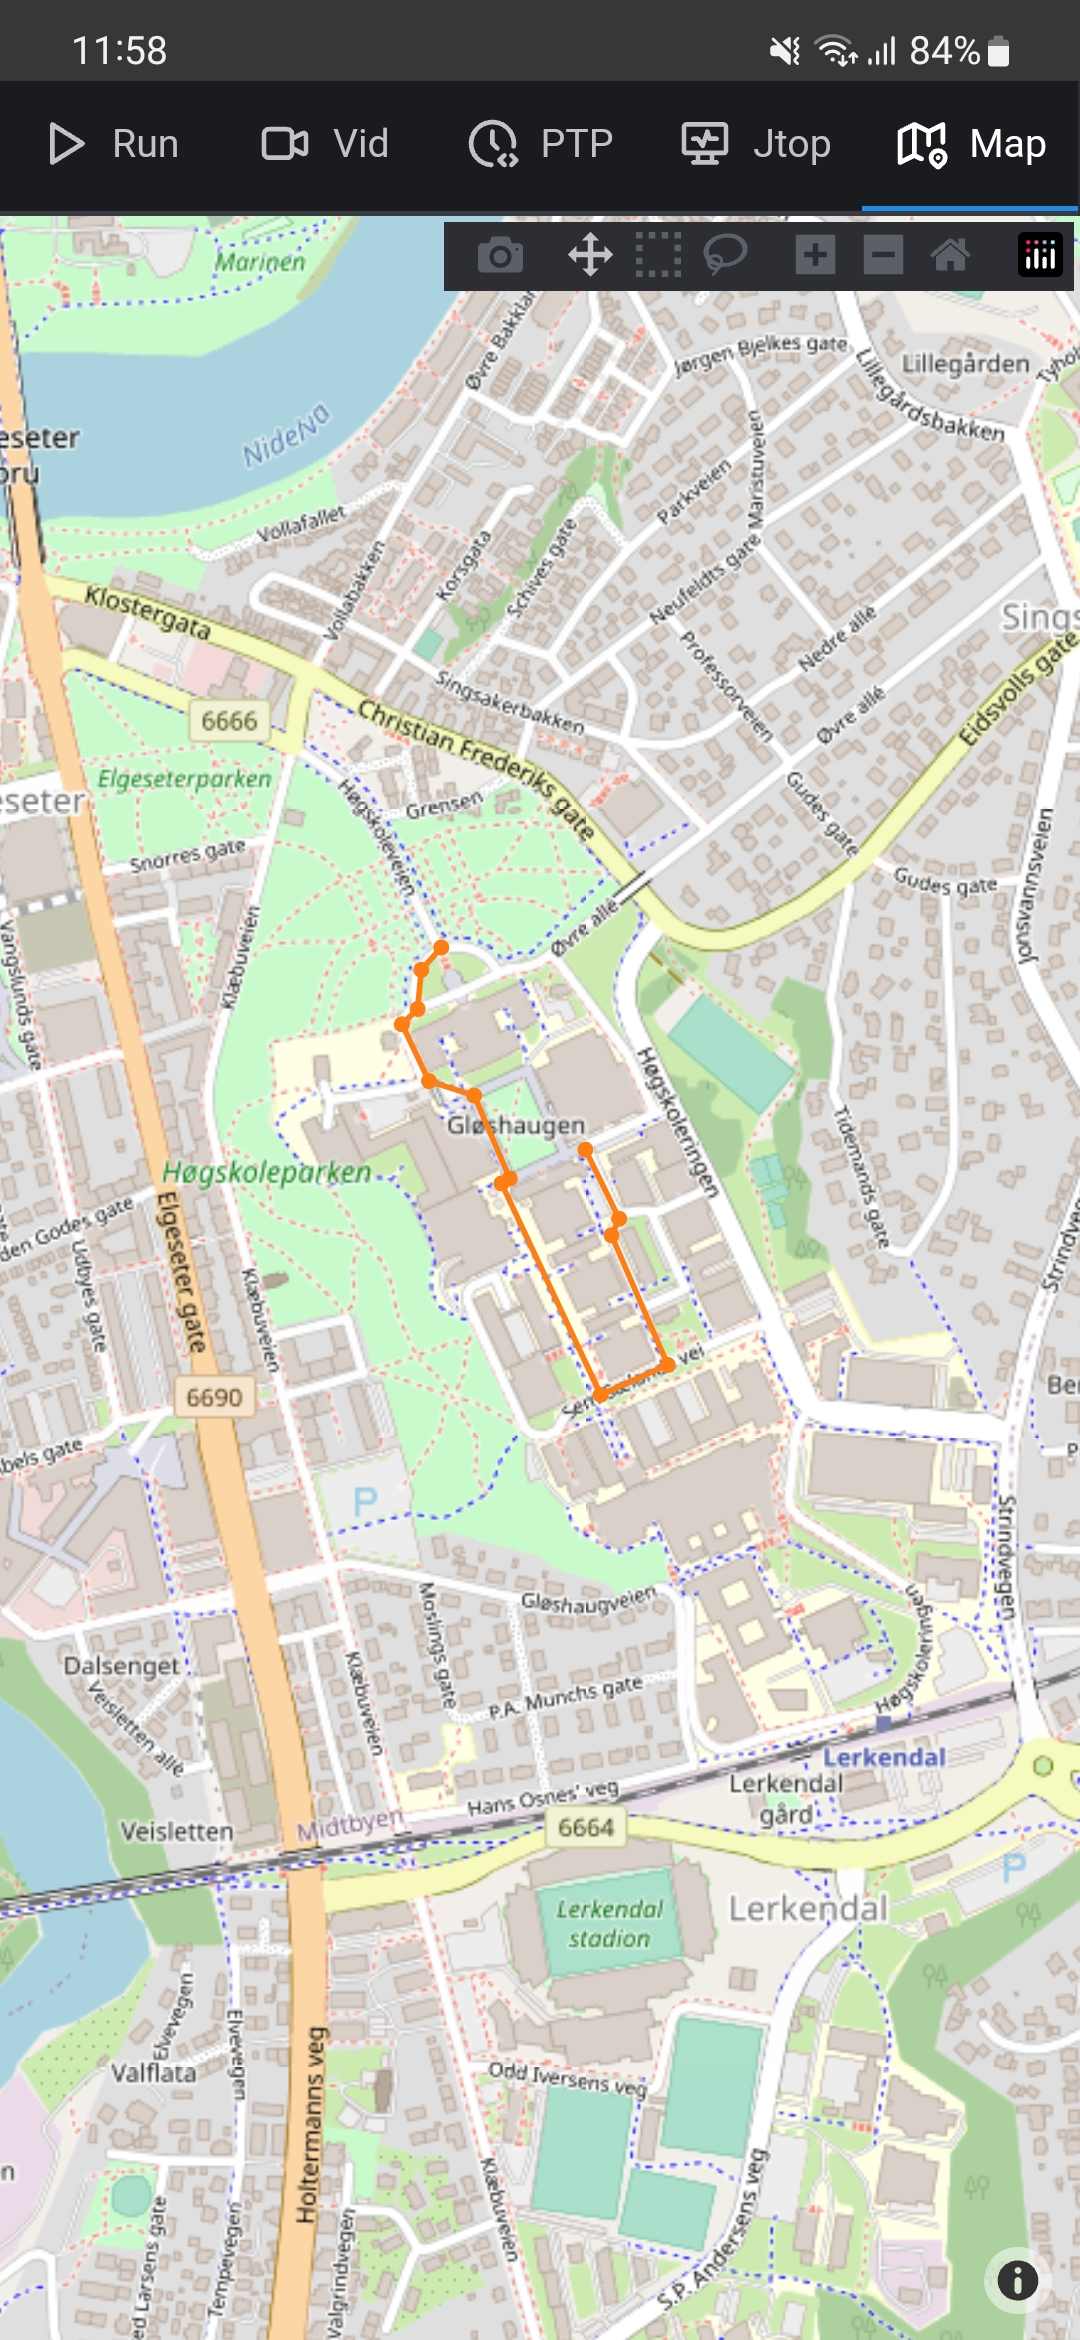
\includegraphics[width=.48\textwidth]{figures/gui/map_map.jpg}
    \caption{Map page of \srgui with and without sattelite overlay showing plottet position data.}
    \label{fig:gui_map}
\end{figure}

To get the sattelite images an intermediate web client that dynamically fetches sattelite images at requested position and zoom level from kartverket was implemented.
The first step is to aquire the \gls{apikey} required to acces the sattelite images as they are not available by default.
It was not easily acessable but after examining the source files of \href{https://www.norgeskart.no}{www.norgeskart.no} were analyzed and the \gls{apikey} was identified as showing up in the \href{https://www.norgeskart.no/norgeskart3-2.0.72.js}{norgeskart3-2.0.72.js} source file and can be found with this regex \code{(?<=gatekeeper.py\?key=)\w+}.
The \gls{apikey} changes periodically but can be stored in the client session to avoid aquiering it for every sattelite image.
With the \gls{apikey}, the client can acces the sattelite images from Kartverket and render them as an overlay in the map.

One minor issue with the sattelite images from Kartverket, is that a white image is returned if the zoom level is to high, which even happens on their own website as shown in Figure \ref{fig:norgeskart_bug}.
The intermediate client solves this by ignoreing those images and returning a \code{404 not found} for those images.

The \gls{apikey} is publically available, but does not appear to be intended for this type of \gls{api} access as it is located deep within the source code of the website.
In the future it might be better to request a proper \gls{apikey} from Kartverket or use a different \gls{api} for sattelite images.

\begin{figure}[H]
    \centering
    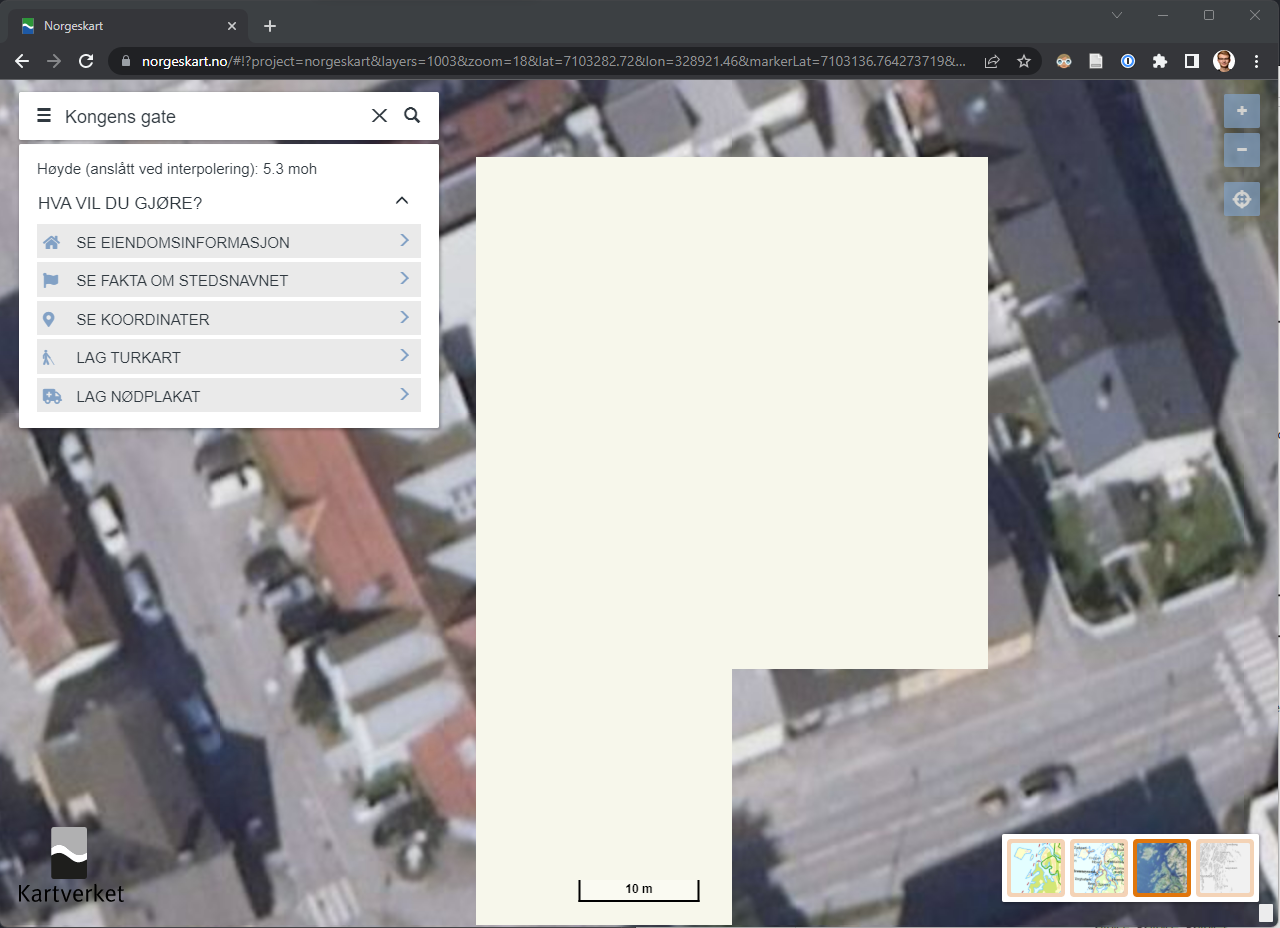
\includegraphics[width=.8\textwidth]{figures/gui/norgeskart_bug.png}
    \caption{Screenshot showing the white patches that appears when zoom level goes beyong 19 \cite{kartverketNorgeskart}}
    \label{fig:norgeskart_bug}
\end{figure}
